\documentclass[notheorems]{beamer}
\usetheme{Lab2C}
\usepackage{graphicx}
\usepackage{subcaption}
\input{macros.tex}
\newif\ifbeamer
\beamertrue

\title{Info-Detection: An Information-Theoretic Approach to Detect Outlier}
\author{Feng Zhao\inst{1} \and Fei Ma\inst{2}\and Yang Li\inst{2} \and Shao-Lun Huang\inst{2} \and Lin Zhang \inst{1,2}}
\institute{\inst{1}Dept. of Electronic Engineering, Tsinghua University
\and \inst{2}Tsinghua-Berkeley Shenzhen Institute, Tsinghua University}
\date{\today}
\begin{document}
\begin{frame}
	\titlepage
\end{frame}
\section*{Outline}
\begin{frame}
	\tableofcontents
\end{frame}

\section{Introduction}
\subsection{Outlier detection and existing method}
\begin{frame}
\frametitle{Outlier detection}
	\begin{columns}
		\column{5cm}
		\begin{figure}
			\includegraphics[width=4cm]{pic/outlier_detection_intro.png}
		\end{figure}
		\column{5cm}
		Outlier detection is the identification of abnormal data which differs from the majority of the data.
	\end{columns}
\begin{figure}
	\centering
	\begin{subfigure}{0.33\textwidth}
		\includegraphics[width=\textwidth]{pic/fraud_detection.jpg}
		\caption{Fraud Detection}
	\end{subfigure}~~~~~
	\begin{subfigure}{0.33\textwidth}
		\includegraphics[width=\textwidth]{pic/activity_monitoring.jpg}
		\caption{Activity Monitoring}
	\end{subfigure}
\end{figure}  
\end{frame}
\begin{frame}
\frametitle{Existing Method}
\begin{figure}
	\centering
	\begin{subfigure}{0.33\textwidth}
		\includegraphics[width=\textwidth]{pic/lof.png}
		\caption{Local Outlier Factor}
	\end{subfigure}~
	\begin{subfigure}{0.58\textwidth}
		\includegraphics[width=\textwidth]{pic/if.png}
		\caption{Isolation Forest}
	\end{subfigure}
\end{figure}  
	\begin{columns}
\column{0.4\textwidth}
\begin{figure}
		\includegraphics[width=4.5cm]{pic/one_class_svm.png}
		\caption*{ \textcolor{thupurple}{(c)} One class SVM}
\end{figure}
\column{0.6\textwidth}
\quad Shortcomings:
\begin{itemize}
\item the number of outliers needs to known 
\item hyperparameters matter
\end{itemize}
\end{columns}
\end{frame}
\subsection{Related work}
\begin{frame}
	\frametitle{Related work}
\begin{itemize}
\item Cluster based method
	\begin{enumerate}
		\item Campello et al. in 2015 proposed a hierarchical density estimate method
%to do outlier detection
		\item Nagano et al in 2010 proposed a minimum average cost clustering method
%which shares the same hierarchical clustering structure with info-clustering.
		\item Chan C et al. in 2016 proposed info-clustering method
%which is a hierarchical clustering method.
	\end{enumerate}
\item Graph partition algorithm
\begin{enumerate}
\item Narayanan in 1991 proposes an algorithm to compute the principal sequence of partition
\item Kolmogorov in 2010 proposes a parametric algorithm for the same task.
\end{enumerate}
\end{itemize}
Our work
\begin{itemize}
\item Info-Detection method
\item Improved algorithm for principal sequence of partition
\end{itemize}
\end{frame}
\section{Formulation of Info-Detection}
\subsection{Info-Clustering}
\begin{frame}
\frametitle{Review of Info-Clustering}
\begin{enumerate}
\item directed graph $G(V, E)$; Node set $Z_V=\{Z_i | i \in V\}$
\item partition $\P=\{C_1, \dots, C_k\}, \bigcup_{i=1}^k C_i = V$ and $i\neq j \Rightarrow C_i \cap C_j = \emptyset$
\item $\Pi$ is the collection of all partitions of $V$, $\Pi' = \Pi \backslash \{V\}$
\item $f(\cdot)$ is the graph in-cut function, $f(C)=\sum_{i \neq C, j\in C, (i,j) \in E} w_{ij}$
\item $f[\cdot]$ is a function defined on $\Pi$ by $f[\P]=\sum_{C\in \P}f(C)$
\end{enumerate}
\begin{definition}[info-cluster]
Given $G(V, E)$, the cluster set $C_{\gamma}(Z_V)$ is defined as 
\begin{align}
I_{\mathcal{P}}(Z_V) & = \frac{f[\P]}{ \abs{\mathcal{P}} - 1}\\
I(Z_V) & = \min_{\mathcal{P} \in \Pi'(V)} I_{\mathcal{P}}(Z_V) \\
C_{\gamma}(Z_V) & := \textrm{maximal}\{ B \in V \vert \, \abs{B} > 1, I(Z_B) > \gamma \}
\end{align}
\end{definition}
\end{frame}
\begin{frame}{Review of Info-Clustering}
\begin{enumerate}
\item  every two sets $C(Z_V)=\bigcup_{\gamma \geq 0} C_{\gamma}(Z_V)$ are either disjoint or have subset relationship
\item sets from $C(Z_V)$ can be arranged in a clustering tree $\mathcal{T}$; The leaf node of $\mathcal{T}$ is $\{j\}$.
\item the largest threshold value $\gamma_N = \max_{A\subseteq V, \abs{A}>1} I(Z_A)$; The maximal set to achieve this is denoted $B$; $\gamma_N = I(Z_B)$.
\end{enumerate}
Example
\begin{columns}
\column{0.45\textwidth}
\begin{figure}
		\includegraphics[width=4.5cm]{pic/example_directed.eps}
\end{figure}
\column{0.55\textwidth}
	\begin{equation*}
	C_{\gamma}(Z_V)	=\begin{cases}
					\{\{1,2,3\}\} & \gamma < 2 \\
					\{\{1,3\}\} & 2\leq \gamma < 5 \\
					\emptyset & \gamma \geq \gamma_N = 5
		\end{cases}
	\end{equation*}
\end{columns}
\end{frame}
\subsection{Info-Detection}
\begin{frame}
	\frametitle{Info-Detection Method}
\begin{itemize}
\item For $\gamma_N = I(Z_B)$, nodes in $B$ are inliers and nodes in $V\backslash B$ are outliers.
\item The ourlier score $Z_j$ for $j \in V\backslash B$ is measured with the depth of the set $\{j\}$ in the hierarchical tree.
\end{itemize}
Example
	\begin{figure}
		\centering
		\includegraphics[width=9cm]{pic/outlier_example.eps}
		\caption*{Info-Detection applied to 6 points on Cartesian plane, with $w_{ij} = \exp(-d_{ij}^2)$}\label{fig:ex}
	\end{figure}
\end{frame}
\begin{frame}{Prediction Scheme for Info-Detection}
For newly added node $i'$. Let $V'=B\cup \{i'\}$, we can compute $\gamma'_N$ for $G(V', E(V'))$.
$ \gamma'_N > \gamma_N \iff i'$ is normal observation. We found that
\begin{proposition}
\begin{equation}
\gamma'_N > \gamma_N \iff  \sum_{i \in B} w_{ii'} > \gamma_N 
\end{equation}
\end{proposition}
\begin{figure}
	\centering
	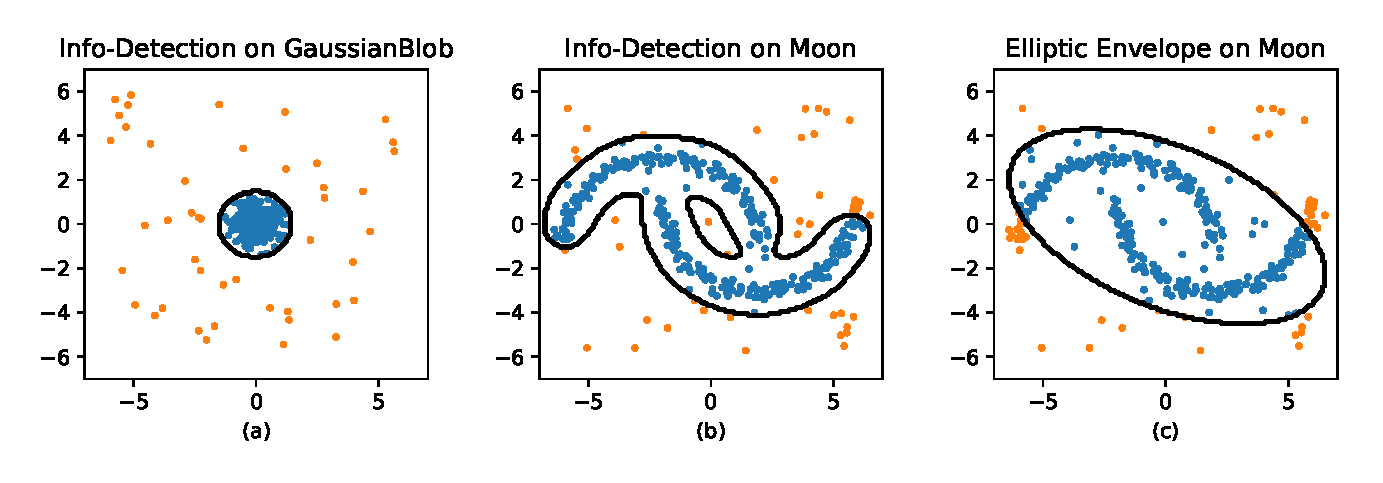
\includegraphics[width=\textwidth]{pic/outlier_boundary_illustration.eps}
	\caption*{Detection boundary lines}	\label{fig:boundary}
\end{figure}
\end{frame}

\section{Algorithms}
\frame{\tableofcontents[currentsection]}
\begin{frame}{Review of Principal Sequence of Partition}
It has been found the mathematical structure of info-clustering is the same with that of principal sequence of partition.
\begin{definition}[Principal Sequence of Partition]
\begin{align}
h_{\P}(\lambda) &=  f[\P] - \abs{\P} \lambda  \label{eq:hPL}\\
h(\lambda) &= \min_{\P \in \Pi'(V)} h_{\P}(\lambda) \label{eq:hLambda}
\end{align}
The optimal partitions $\P_1, \dots, \P_k$ for $h(\lambda)$ are nested such that $\P_1 \succeq \P_2 \dots \succeq \P_k$,  which are called principal sequence of partition (PSP) of the graph $G$.
\end{definition}
We call $\lambda^*$ a critical value for PSP if $\P_i, \P_{i+1}$ are both minimizer for $h(\lambda^*)$ in \eqref{eq:hLambda}.
The largest critical value is equal to $\gamma_N$ and the largest set in $\P_{k-1}$ is equal to $B$.
\end{frame}
\begin{frame}
\frametitle{Review of Narayanan's Algorithm to compute PSP}
\begin{columns}
\column{0.5\textwidth}
\algsetup{linenosize=\tiny}
\begin{algorithm}[H]
\caption*{Narayanan's Algorithm}\label{alg:psp}
{\tiny
\begin{algorithmic}[1]
\REQUIRE a directed graph $G(V,E)$
\ENSURE A sorted critical value array \textbf{L} and a reverse ordered array \textbf{PSP} containing $\P_1,\dots, P_k$.
\STATE \textbf{L}  $\leftarrow$ empty list.
\STATE $Q\leftarrow \{V\}, P \leftarrow \{ \{i \} | i \in V\}$
\STATE $\mathbf{PSP}= [Q, P]$
\STATE \texttt{Split}$(Q,P)$
\STATE sort $L$ and sort $\mathbf{PSP}$ with respect to $\succeq$ 
\FUNCTION{\texttt{Split}$(Q,P)$}
 \STATE\label{alg:gamma} $\gamma' = {1 \over \abs{P} - \abs{Q}} (f(P)-f(Q))$
 \STATE $h' = {1 \over \abs{P} - \abs{Q}}(\abs{P} f(Q) - \abs{Q} f(P))$
 \STATE $(\tilde{h}, P') = \texttt{DT}(f,\gamma')$
 \IF{$\tilde{h} = h'$}
 	\STATE insert $\gamma'$ to $\mathbf{L}$
 \ELSE
 	\STATE insert $P'$ to $\mathbf{PSP}$
 	\STATE \texttt{Split}$(Q, P')$
 	\STATE \texttt{Split}$(P',P)$
 \ENDIF
\ENDFUNCTION
\end{algorithmic}
}
\end{algorithm}
The whole graph $G$ is used in each compution of \texttt{DT} routine.
\column{0.5\textwidth}
\begin{figure}
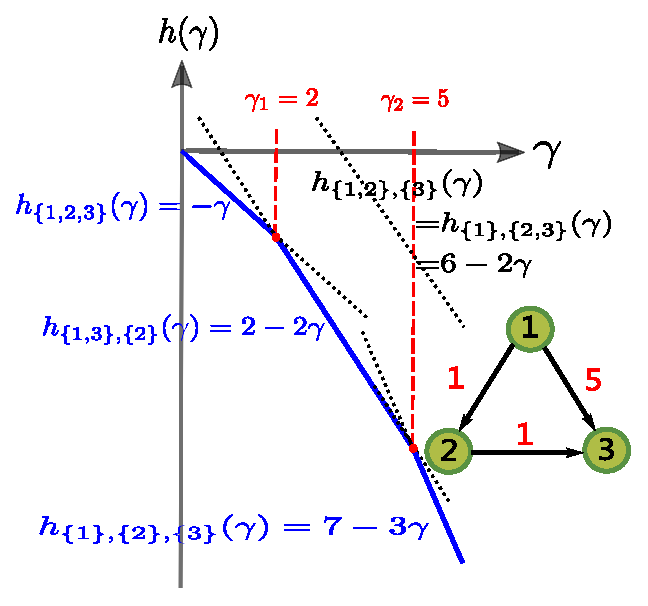
\includegraphics[width=4.5cm]{pic/dt_with_graph.eps}
\end{figure}
\begin{align*}
\P_0  & = \{\{1,2,3\}\} \\
\P_1  & = \{\{1,3\},\{2\}\} \\
\P_2  & = \{\{1\},\{2\},\{3\}\} 
\end{align*}
\end{columns}
\end{frame}
\begin{frame}
\frametitle{Improved PSP Algorithm}
\begin{columns}
\column{0.5\textwidth}
\vskip -1.2em
\algsetup{linenosize=\tiny}
\begin{algorithm}[H]
\caption*{{\footnotesize Improved PSP Algorithm}}
{\tiny
	\begin{algorithmic}[1]
		\REQUIRE a directed graph $G(V, E)$
		\ENSURE a hierarchical tree $\mathcal{T}(K, E)$ where $K \subseteq 2^{V}$ is node set and $E$ is edge set.
		\STATE initialize tree $\mathcal{T}$ with $V$ as root node, $\{j\}(j\leq \abs{V})$ as leaf node and no stem node.
		\STATE \texttt{Split}($G, V$)
		\FUNCTION{\texttt{Split}($\widetilde{G}, \widetilde{V}$)}
		\STATE $w$ is the summation of all edge weights of $\widetilde{G}$ 
		\STATE $\gamma' = \frac{w}{\abs{V(\widetilde{G})}-1}$ where $V(\widetilde{G})$ is node set of graph $\widetilde{G}$ \label{alg:gamma_apostrophe}
		\STATE $(\tilde{h}, P') = \texttt{DT}(\widetilde{G}, \gamma')$ 
		\IF{$\tilde{h} = - \gamma'$}
		\STATE add edge weight $\gamma'$ in $\mathcal{T}$ starting from $\widetilde{V}$ to its children.
		\ELSE
		\FOR{$S$ in $P'$ and $\abs{S}>1$}
		\STATE make children of $\widetilde{V}$ in $\mathcal{T}$ have new parent $S$		
		\STATE make the parent of $S$ be $\widetilde{V}$
		\STATE \texttt{Split}($\widetilde{G}[S], S$) where $\widetilde{G}[S]$ is the subgraph of $\widetilde{G}$ restricted on $S$
		\STATE contract $S$ to a single node in $\widetilde{G}$ % graph \widetilde{G} is modified
		\ENDFOR 
		\STATE \texttt{Split}($\widetilde{G}, \widetilde{V}$)		
		\ENDIF
		\ENDFUNCTION
	\end{algorithmic}
}
\end{algorithm}
\vskip -1.2em
Smaller graph $G$ is used in each compution of \texttt{DT} routine.
\column{0.5\textwidth}
\begin{figure}
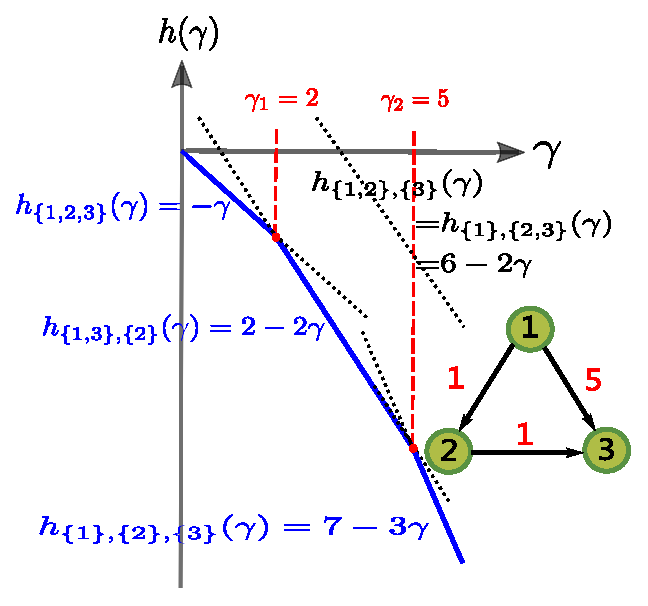
\includegraphics[width=4.5cm]{pic/dt_with_graph.eps}
\end{figure}
\begin{align*}
\P_0  & = \{\{1,2,3\}\} \\
\P_1  & = \{\{1,3\},\{2\}\} \\
\P_2  & = \{\{1\},\{2\},\{3\}\} 
\end{align*}
\end{columns}
\end{frame}

\begin{frame}
	\frametitle{Solving $\min_{t\in C} \{f(C) - \lambda - y^{\lambda}(C)\}$}
	\begin{columns}
    \column{5.3cm}
    \begin{itemize}
	\item $y^{\lambda}$ is a vector
	\item $y^{\lambda}_i = \min\{a_i - \lambda, b_i\}$ 
	\item $y(C) = \sum_{i \in C} y_i$	
	\item $g_{\lambda}(T) = f(T) - \lambda - y^{\lambda}(T)$
	\item $T^{\lambda} = \argmin_{t\in V} g_{\lambda}(T)$
	\end{itemize}
	\begin{theorem}[Principal Sequence]
		\begin{align}\notag
			T^{\lambda} & =\begin{cases}
				T_0 & \lambda < \lambda_1 \\
				T_i & \lambda_i \leq \lambda < \lambda_{i+1}\\
				T_k & \lambda \geq \lambda_{k}
			\end{cases} \\
				T_k & \subsetneq  \dots \subsetneq T_1 \subsetneq T_0 \label{eq:Alambda}				
		\end{align}
    \end{theorem}
	\column{4.7cm}
	\algsetup{linenosize=\tiny}
	\input{alg_parametric_computing.tex}	
    \end{columns}
\end{frame}
\begin{frame}
	\frametitle{Illustrative Example}
\begin{columns}
	\column{5cm}
	\begin{figure}
		\includegraphics[width=5cm]{pic/example_pst_single.eps}
		\caption{parametric computing illustration}
	\end{figure}
	\column{5cm}
	\begin{align*}
	\tilde{h}(\lambda) &= \min_{t \in T} g_{\lambda}(T)\\
	t & = 3 \\
	y^{\lambda}_i & = -\lambda, i=1,2,3 \\
    \mathbb{L} & = [1, 5, +\infty] \\
	T^{\lambda} &= [\{1,2,3\}, \{1,3\}, \{3\}]
	\end{align*}
\end{columns}	
\end{frame}	
\begin{frame}
	\frametitle{Converting to maximum flow problem}
\begin{columns}
	\column{4cm}
	\begin{figure}
		\includegraphics[width=4cm]{pic/example_st.eps}
		\caption{graph $\widetilde{G}$}
	\end{figure}
	\column{6cm}
	\begin{align*}
		& c^{\lambda}(i, j)  = \\ 
		& \begin{cases}
			\max\{0, -y^{\lambda}_i\} &  i = s, j \neq t \\
			w_{it} + \max\{0, y^{\lambda}_i\} & i\neq s, j = t\\
			0 & i = s, j = t\\
			w_{ij} & i \neq s, j \neq t
		\end{cases}
	\end{align*}
\end{columns}	
Minimizing $g_{\lambda}(T)$ is equivalent to solve the maximum flow for $\widetilde{G}$.
\end{frame}	

\section{Experiment}
\frame{\tableofcontents[currentsection]}
\begin{frame}
	\frametitle{How to choose graph weight}
	\framesubtitle{preliminary result}
	\begin{proposition}
		\begin{itemize}
			\item The clustering tree has no stem nodes if and only if
			\begin{equation}
			\frac{f[\P]}{\abs{\P}-1} \geq \frac{\sum_{(i,j) \in E} w_{ij}}{\abs{V}-1}				
			\end{equation}
			holds for any partition $\abs{\P} > 1$.
			\item Let $w_{ij}=0$ if $(i,j)\not\in E$. If $w_{ij} + w_{jk} \geq w_{ki}$ for any different triple $i, j, k \in V$, then the clustering tree has no stem nodes.
			\item Suppose $S_1, S_2 $ are complete graph with size $n$ equal weight $w_{ij}=n$. There are $m$ edges between the two graphs and all inter-connection edges have equal weight 1. Then for $V=S_1\cup S_2$, we have
			\begin{equation}
				I(Z_V) = \begin{cases}
					m & m <\frac{n^2}{2}, S_1,S_2 \textrm{ are non-trivial cluster} \\
					\frac{m+n^2(n-1)}{2n-1} & m\geq \frac{n^2}{2}, \textrm{ only trivial cluster exists} 
				\end{cases}
			\end{equation}
				
		\end{itemize}
	\end{proposition}
\end{frame}
\begin{frame}
\begin{figure}[!ht]
\begin{subfigure}{\textwidth}
\centering
\IfFileExists{experiment/data_clustering/plot_art/build/4part.eps}
{\includegraphics[width=11cm]{experiment/data_clustering/plot_art/build/4part.eps}}
{\includegraphics[width=12cm]{pic/4part.eps}} % not up-to-date

\caption{Illustrative example from four Gaussians}\label{fig:4p}
\end{subfigure}
\begin{subfigure}{\textwidth}
\centering
\IfFileExists{experiment/data_clustering/plot_art/build/3circle.eps}
{\includegraphics[width=11cm]{experiment/data_clustering/plot_art/build/3circle.eps}}
{\includegraphics[width=12cm]{pic/3circle.eps}} % not up-to-date
\caption{Illustrative example from three circles}\label{fig:3c}
\end{subfigure}
\end{figure}
\end{frame}
\begin{frame}
\frametitle{empirical comparison}
\begin{table}[!ht]
\centering
\InputIfFileExists{compare_3.tex}{}{}
\caption{clustering accuracy for info-clustering and existing algorithms}
\end{table}
\end{frame}
\begin{frame}
\frametitle{Info-clustering in hierarchical community detection problem}
\begin{figure}
	\centering
	\begin{subfigure}{0.45\textwidth}
		\includegraphics[width=\textwidth]{pic/two_level.eps}
		\caption{a community with two hierarchical levels}\label{fig:c1}
	\end{subfigure}
	\begin{subfigure}{0.45\textwidth}
		\includegraphics[width=\textwidth]{pic/tree_info-clustering.pdf}
		\caption{hierarchical tree obtained by graph-based info-clustering for left figure. The tree leaves with the same ancestor are merged for clarity.}\label{fig:c2}
	\end{subfigure}
	\caption{Community Detection Experiment Illustration}
\end{figure}
\end{frame}
\begin{frame}
	\begin{block}{model parameter}
	\begin{description}
	  \item[$z_{\mathrm{in}_1}$] average node degree within micro community;
	  \item[$z_{\mathrm{in}_2}$] average node degree between different micro communities but within one macro community;  
	  \item[$z_{\mathrm{out}}$] average node degree between different macro communities
    \end{description}
    Robinson-Foulds distance measure between two trees;    
    {\footnotesize compared with GN(Girvan-Newman) and BHCD(Bayesian hierarchical community detection).
	}
    \end{block}
\begin{figure}
	\centering
	\begin{subfigure}{0.33\textwidth}
		\includegraphics[width=\textwidth]{pic/z_in_1.eps}
		\caption{}
	\end{subfigure}~
	\begin{subfigure}{0.33\textwidth}
		\includegraphics[width=\textwidth]{pic/z_in_2.eps}
		\caption{}
	\end{subfigure}~
	\begin{subfigure}{0.33\textwidth}
		\includegraphics[width=\textwidth]{pic/z_o.eps}
		\caption{}
	\end{subfigure}
	\caption{{\scriptsize Distance comparison between different hierarchical community detection method.}}\label{fig:cdr}	
\end{figure}    
\end{frame}
\section{Conclusion and Contribution}
\begin{frame}
\frametitle{Conclusion}
\begin{itemize}
\item propose graph-based info-clustering method
\item propose a parametric computing scheme to get the hierarchical structure of given graph 
\item apply graph-based info-clustering to cluster dataset and find structure of community
\end{itemize}
\end{frame}
\section{Reference}
\begin{frame}
\frametitle{Reference}
\begin{thebibliography}{9}
\bibitem{ic} Chung Chan, \newblock Info-Clustering: A Mathematical Theory for Data Clustering
\newblock  IEEE Transactions on Molecular, Biological and Multi-Scale Communications, June 2016
\bibitem{pin}  Chung Chan, \newblock Info-Clustering: An Efficient Algorithm by Network Information Flow
\newblock 2017 Information Theory and Applications Workshop (ITA)
\bibitem{mac} Kiyohito Nagano \newblock Minimum Average Cost Clustering \newblock NIPS 2010
\bibitem{RN4}
Vladimir Kolmogorov.
\newblock A faster algorithm for computing the principal sequence of partitions
of a graph.
\newblock {\em Algorithmica}, 56(4):394--412, 2010.
\end{thebibliography}
\end{frame}
\end{document}
